% !TeX spellcheck = en_UK
\chapter{Background} \label{background}

\section{Colorectal Polyps, Medical Imaging, and Deep Learning}
	Polyps are small growths found in and around the inner lining of the large intestine. These polyps, also referred to as adenomas, can in time develop into cancerous tumours, or carcinomas, in a process known as the adenoma-carcinoma sequence \cite{ACS}. Though the majority of polyps do not undergo this process, identifying polyps nonetheless constitutes an important step towards preventing colorectal cancer. Indeed, resection of these polyps has been shown to reduce the incidence of colorectal cancer by a significant margin \cite{resection}. 
	
	Though colorectal cancer remains as one of the leading causes of cancer-related death worldwide \cite{colorectal_cancer}, mortality rates have in recent years declined in large part to the increased use of screening colonoscopy and subsequent preemptive treatment \cite{screening}. Polyps are by nature somewhat difficult to detect, however, and are routinely missed by clinicians, with miss rates reportedly ranging upwards of 27\% for diminutive (<2.5mm) polyps \cite{missrate1, missrate2}.
	
	Reducing this miss rate has the potential to further reduce the incidence of colorectal cancer. As a result, there has been a significant body of work dedicated to developing systems and techniques to aid in more accurate screening. Certain image-processing techniques, namely I-SCAN, have for instance been shown to reduce miss-rates by up to 50\% \cite{i-scan}. Similarly, the use of narrowband imaging, wherein light of specific wavelengths specifically designed to highlight the textural differences between the polyps and the surrounding tissue, have been shown to reduce miss rates by 26\% \cite{nbi}. 
	
	These systems do, however, require specialized equipment, training and expertise to effectively employ. Thus, automatic polyp segmentation using deep neural networks (DNNs), and in particular convolutional neural networks (CNNs), has also been identified as a possible auxiliary detection method. Such CNN-aided endoscopy requires minimal training time on the part of the clinician, no additional equipment, and has been shown to increase detection rates by 10\% when deployed in a clinical setting \cite{polyp-success-story}. 

	This has spurred on a large body of research dedicated to improving the performance and expanding the capabilities of deep-learning based systems for polyp detection and segmentation. Several challenges been also held, namely the Endotect Challenge \cite{endotect}, EndoCV2020 \cite{endocv2020} and EndoCV2021 \cite{endocv2021}.
	
	There are, however, still several hurdles to overcome; recent research has shown that even state of the art deep-learning pipelines are prone to generalization failure when deployed in practical settings, particularly when exposed to distributional shifts such as changes in demographics, imaging equipment, noise, and more despite exhibiting high performance on hold-out sets \cite{retinopathy, damour2020underspecification, pneumonia, shortcut_learning}. This was further highlighted in the EndoCV2021 challenge, wherein submissions were evaluated on a hidden dataset collected from a different hospital than the training data. The results from this challenge demonstrated the pervasiveness of generalization failure, with every submitted model exhibiting significant performance reductions when evaluated on the hidden dataset \cite{endocv2021}. 
	
	Naturally, automatic segmentation systems are rendered practically useless should they fail to perform sufficiently outside the very carefully controlled conditions within which typical deep learning models are developed. Increasing the generalizability of the deep learning pipeline is as a result of significant interest. 

\section{Generalization Failure in the Wild} \label{case_studies}
	\subsection{Generalization Failure in Medical Imaging}
	Generalization failure is not, of course, unique to the polyp segmentation. Though medical imaging has in recent years proven to be one of the most promising applications of artificial intelligence and deep learning, having the capacity to significantly improve both the accuracy and efficiency of detection, diagnosis, and treatment of a wide variety of diseases \cite{dl_medical_imaging}, medical deep learning systems are nonetheless highly prone to generalization failure \cite{damour2020underspecification, shortcut_learning}.
	
	For instance, a deep-learning based classifier which successfully detected pneumonia in X-ray scans across a number of hospitals with striking accuracy was determined to be basing its predictions not on any lesions or otherwise pathologically relevant features in the images, but rather on a hospital-specific metal token that could be found in every image, which it used in conjunction with learning the pneumonia prevalence rate of for the respective hospitals to make predictions. As a result, when deployed on data from hospitals that it had not seen during training, the system failed to generalize \cite{pneumonia}. In another study, it was shown that a classifier intended to detect diabetic retinopathy exhibited significant variability in performance depending on the type of camera used \cite{damour2020underspecification}. The same study also showed that similar performance variability could be found when detecting skin-conditions across demographics with differing skin tones. Finally, a model trained to detect and diagnose melanomas  was shown to in large part be basing its predictions on whether it could detect any pre-surgical markings, used by doctors to assist in surgery preparation, in the vicinity of the lesion as opposed to actually learning anything about what the melanomas themselves\cite{skin_shortcut}.  
	 
	\subsection{Generalization Failure in General}
	Though generalization failure is perhaps best represented in medical domains, the phenomenon is pervasive in practically every application of deep learning, albeit to varying degrees. It has for instance been shown that CNNs trained on ImageNet, one of the largest and most diverse datasets in the domain of computer vision, are heavily biased towards textural features, and consequently fail when the texture of the input is modified, despite the shape and structure of the relevant object remaining recognizable\cite{texturebias}. Though this result is based on evaluation on synthetic data, it highlights a key property of deep learning pipelines: namely that they do not necessarily learn features that are causal - in other words, that they are intrinsic to the relevant object - inasmuch as they learn features that are highly correlated - in other words, features that are associated with the object but are not intrinsic to it. Though the texture of cat fur for instance is highly correlated with the "cat" class, it is not the fur that makes the cat. In Figure \ref{cat_elephant}, for instance, it is clear that image (c) should be classified as a cat more than an elephant. Granted, this example is as mentioned fairly synthetic, but a similar situation could arise if the classifier for instance was tested on a black-and-white image of a hairless cat. 
	\begin{figure}[h]
		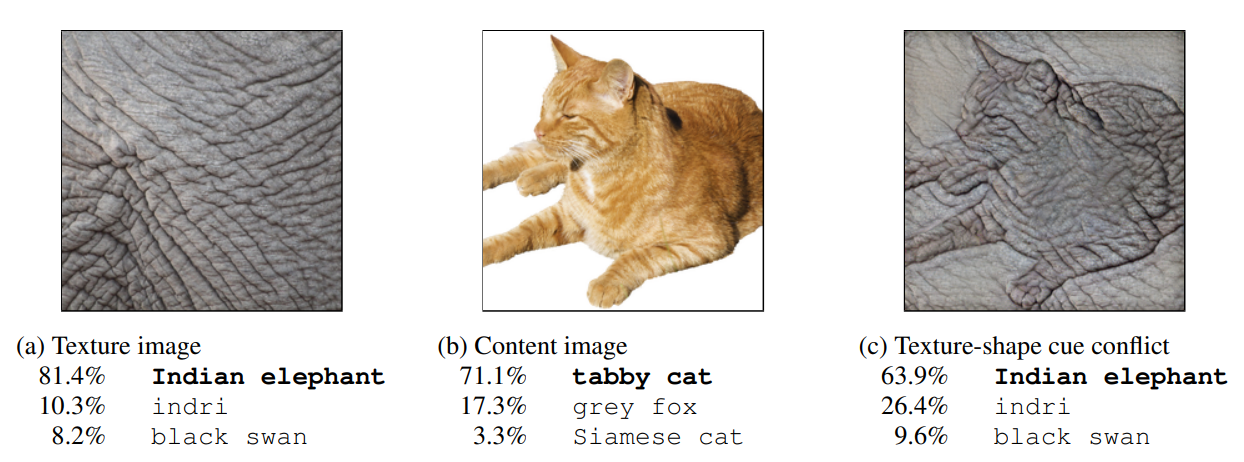
\includegraphics[width=\linewidth]{illustrations/cat_elephant.png}
		\caption{Classifiers trained on ImageNet are biased towards textural features}
		\label{cat_elephant}
	\end{figure}
	
	This behaviour of considering correlations over causation can also be found in state-of-the-art image captioning systems, for instance Microsoft Azure's computer vision API and NeuralTalk2 \cite{electric_sheep}, wherein the model seemingly hallucinates that it sees sheep when evaluated on grassy pastures or hills. Once again, it is of course natural to expect that sheep can be found in these contexts, but it is not these contexts that define what it means to be a sheep. Grassy pastures and sheep are not causally related, only correlated, but deep learning pipelines lack the nuance required to understand this fact. 
	\begin{figure}[h]
		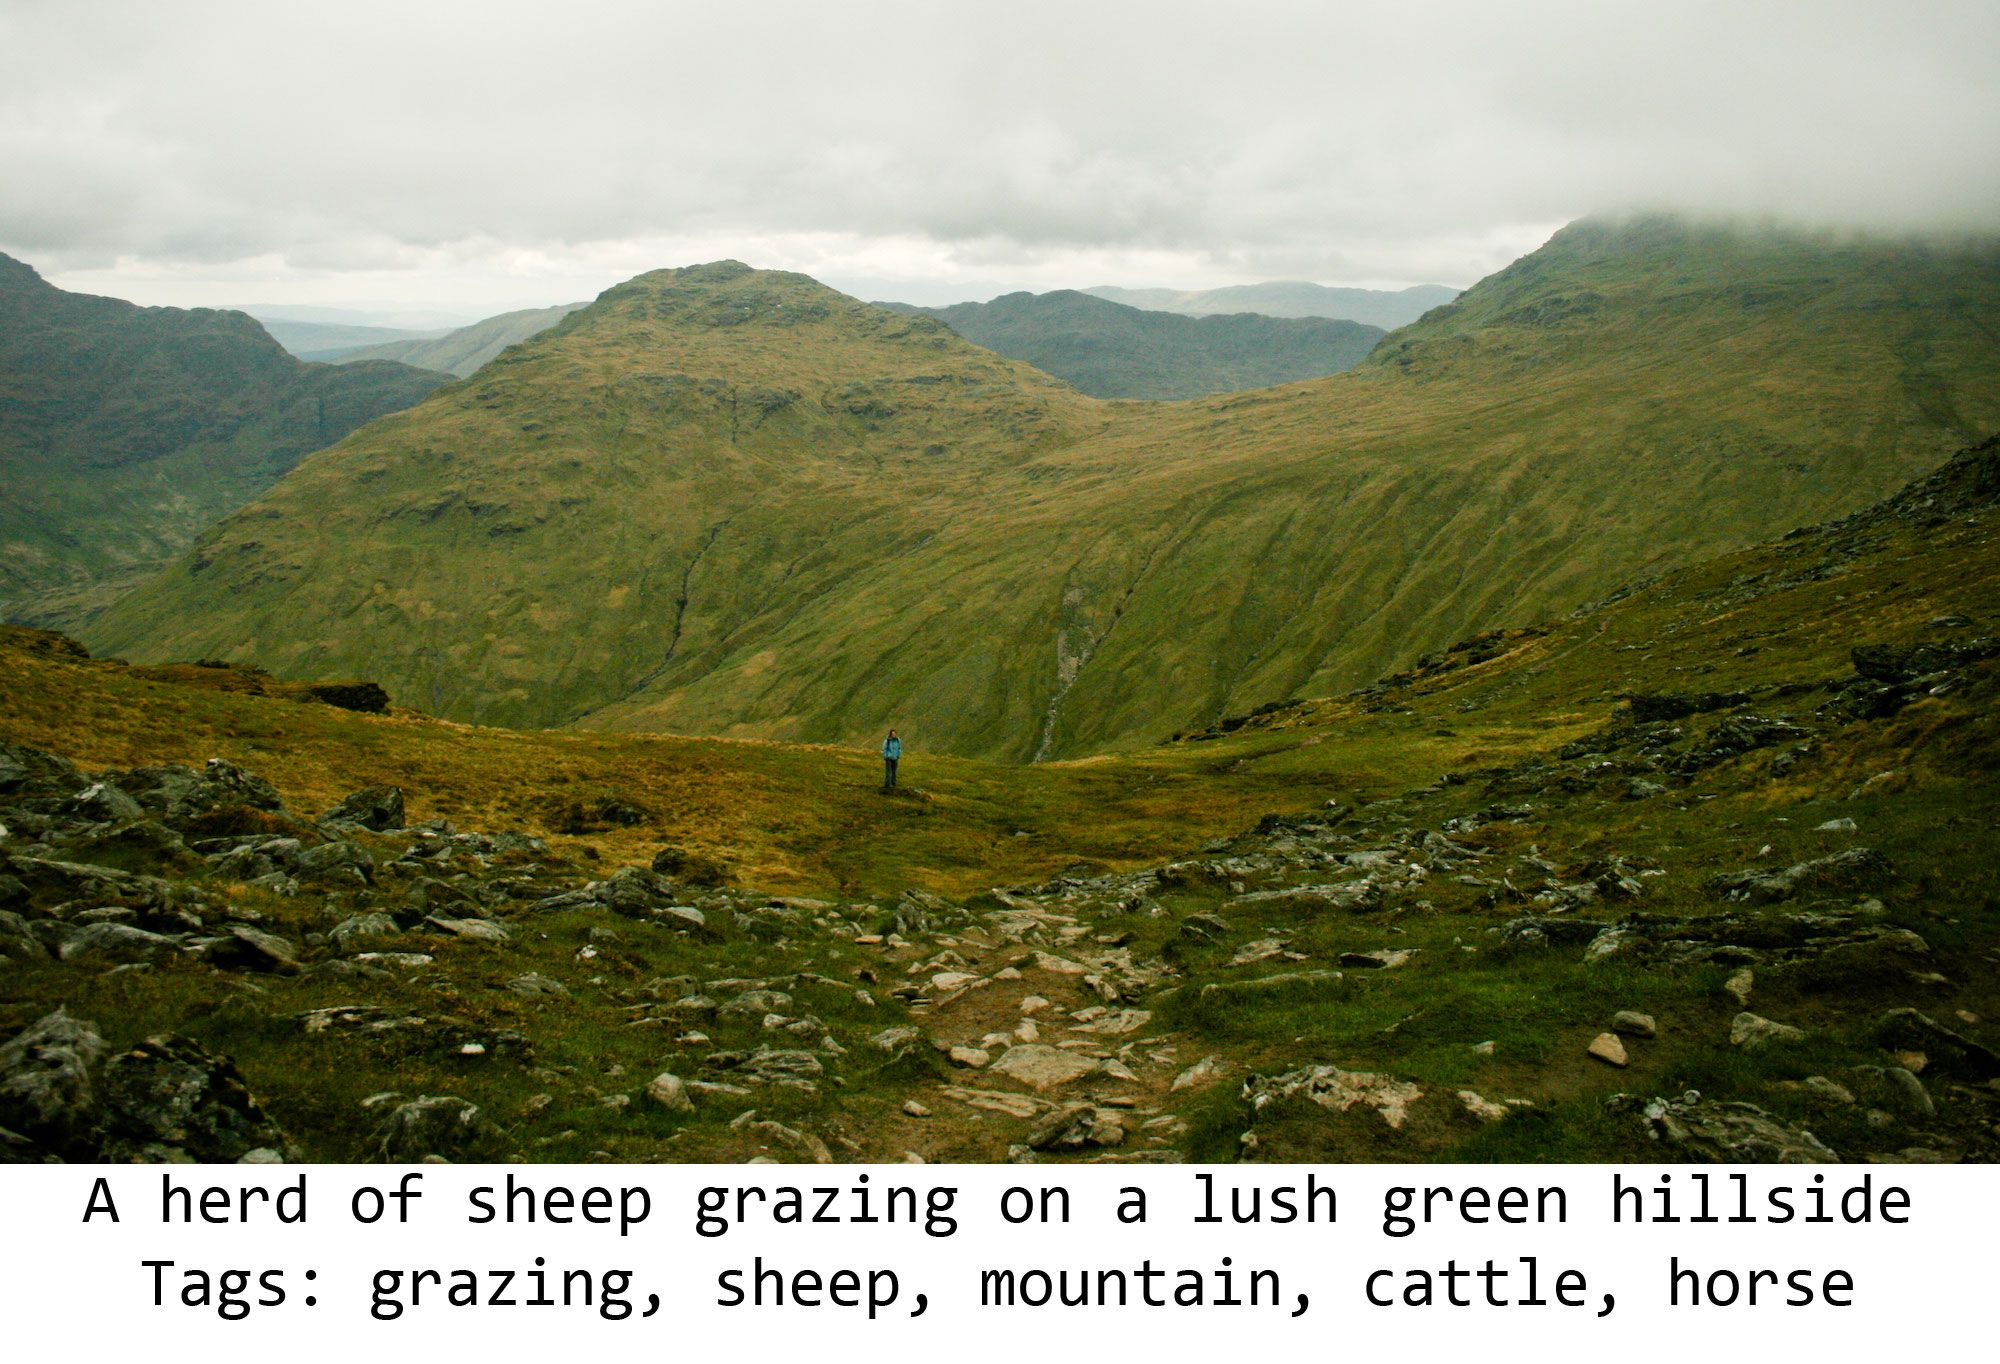
\includegraphics[width=\linewidth]{illustrations/sheep.jpg}
		\caption{Deep captioning models hallucinate sheep when presented with contexts highly correlated with sheep. Adapted from \cite{electric_sheep}}
		\label{sheep}
	\end{figure}


	Another characteristic of deep learning that supports this argument is the effectiveness of adversarial attacks \cite{adversarial_bugs_features}, which specifically target weaknesses in the inductive biases within DNNs through any number of means in an attempt to induce high rates of incorrect, yet highly confident predictions. Gradient-based adversarial attacks, for instance, use the gradients of the model to break even the most sophisticated and well-trained pipelines merely by adding some carefully crafted, yet visually imperceptible noise to the inputs \cite{adversarial_attacks}. Even without access to the gradients, there exists a multitude of so-called black-box attacks that only use output samples to generate similarly effective attacks (cite). Finally, it has been shown that adding minor visual distractions to objects, for example adding bits of tape or graffiti to stop signs, dramatically increases misclassification rates \cite{physical_attacks}. 
	
\section{Generalizability Theory}
	Exactly why and how DNNs seem to so persistently fail to generalize is a topic of ongoing research, and the available literature seems to suggest that the problem is multifaceted. This section is an attempt to summarize and distil the findings and analyses performed in the literature so far. It will cover the theoretical basis of generalization and why one might expect DNNs to generalize, discuss the key characteristics of generalization failure, and finally why and how these characteristics arise with respect to the theory.
	\subsection{Generalization through Empirical Risk Minimization} 
		Naturally, deep learning would not have experienced as much of a revolution in the last decade or so if there was not some semblance of an expectation that their striking performance was generalizable and performant also outside the idealized settings typically involved in research. The theoretical basis that informs this belief in (most) modern deep learning pipelines is the idea of so-called empirical risk minimization, wherein it is assumed that the dataset upon which the model is trained is a representative sample of the distribution of all possible samples in the relevant domain. In other words, it assumes that the dataset is independently and identically distributed (iid) to the domain distribution. To better understand this assumption, it is beneficial to consider it from first principles: 
		
		At the most fundamental level, the goal of machine learning is to learn a mapping between two spaces of objects \(X\) and \(Y\). This mapping, namely the function \(f: X \rightarrow Y\), maps some input object \(x \in X\), an image for example, to a corresponding and application-relevant output object \(y \in Y\), for instance a segmentation mask or class-wise probabilities. It is worth noting, however, that \(f\) is not as much a function in the mathematical sense as much as it is an abstraction of the relationship that the deep learning system is intended to capture. \(f\) cannot as a consequence typically be modelled explicitly. Instead, machine learning systems aim to find a sufficient approximation of this mapping by leveraging a training set \(\{x_i, y_i\}_{0...n}\). This is referred to as supervised learning, and the resulting approximation found using the training set is denoted by \(h: X \rightarrow \hat{Y}\), and typically referred to as a hypothesis.  
		        
		To find such an approximation, we assume that there exists a joint probability distribution over \(X\) and \(Y\), namely \(P(x,y)\), and that the training data \(\{x_i, y_i\}_{0...n}\) is drawn from this probability distribution such that the resulting sample distribution is independent and identically distributed to \(P(x,y)\). This is the so-called iid assumption. By modelling the mapping as a joint probability distribution, one can model uncertainty in the predictions by expressing the output as a conditional probability \(P(y|x)\). In conjunction with a loss-function \(L(h(x),y)\) which measures the discrepancy between the hypothesis and the ground truth, these assumptions allows us to quantify the expected performance of a given hypothesis:
		\begin{equation}
		    R(h) = \mathbb{E}[L(h(x),y)] = \int L(h(x),y) dP(x,y)
		\end{equation}
		Using this framework, one can then find an iid-optimal hypothesis, often called a predictor, by finding the predictor \(h^*\) among a fixed class of functions (defined by network architecture) \(\mathcal{H}\) that minimizes risk:
		\begin{equation}
		h^* = \argmin_{h \in \mathcal{H}}R(h)
		\end{equation}
		
		Since \(P(x,y\)) is not known, however, one cannot compute \(R(h)\) explicitly. Instead, the expected risk has to be estimated empirically, i.e by finding the arithmetic average of the risk associated with each prediction by the hypothesis over the training set:
		\begin{equation}
		R_{emp}(h) = \frac{1}{n}\sum_{i=1}^{n}L(h(x_i), y_i)
		\end{equation}
		This risk can in turn be minimized with respect to the hypothesis class. This is called empirical risk minimization (ERM):
		\begin{equation}
		\hat{h} = \argmin_{h \in \mathcal{H}}R_{emp}(h)
		\end{equation}
		To reiterate, the central idea with this approach to machine learning is that the training data can be considered a finite iid sampling of the underlying distribution. As such, by the central limit theorem, the hold-out performance of the computed hypothesis will approach iid-optimal performance given a sufficient amount of training data and some sufficiently capable training procedure. This should in theory allow deep learning systems to be able to generalize, since the empirical risk in theory can approximate the true risk arbitrarily well given sufficient training data.

		As described in section \ref{case_studies}, ERM nonetheless readily fails to generate generalizable predictors with respect to out-of-distribution data. There are multiple dimensions to this phenomenon, as there are several means by which a model can fail to generalize. To better understand these failure modes, it helps to consider the assumptions that are made in the formulation of ERM, namely that:
		\begin{enumerate}
			\item \(f\) exists in \(\mathcal{H}\) \label{underfit}
			\item The optimal predictor can be found solely through minimizing \(R_{emp}(h)\)\label{overfit}
			\item \(\{x_i, y_i\}\) is an IID sampling of \(P(x,y)\) \label{structural_misalignment}
			\item \(\hat{h}^*\) is unique in \(\mathcal{H}\)\label{underspecification}
		\end{enumerate}
		As the following sections will show, violations of any one of these assumptions can and typically will result in generalization failure. 

	\subsection{Realizability and Underfitting}
		Violations of assumption \ref{underfit} corresponds to a well known and fairly well understood form of generalization failure, namely underfitting. One can however argue that underfitting can be all but discounted as plausible explanation for the pervasiveness of generalization failure observed in modern deep learning pipelines. Underfitting occurs when the model simply lacks the complexity required to encapsulate the patterns necessary to form generalizable interpretations of the data. To give a simple example - consider the problem of trying to fit a linear model to the following dataset: 
		\begin{figure}[h]
			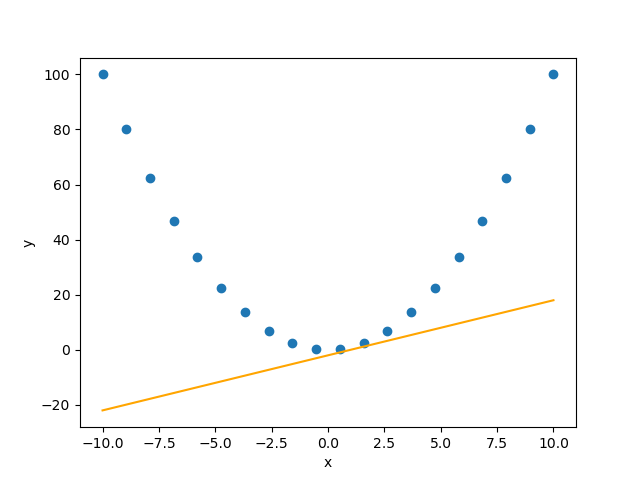
\includegraphics[width=\linewidth]{illustrations/regression_example.png}
			\caption{A linear model cannot fit polynomial data}
			\label{underfit example}
		\end{figure}
		Obviously, no amount of optimization of the parameters in the linear model can ever result in a sufficient description of the underlying data and the function it follows, namely \(y=x^2\). 
		
		This, however, does not necessarily mean that an underfitted model cannot perform well; the above function is after all locally linear, and if it is only evaluated on a limited region, a linear model may perform just fine. One can as such argue that DNNs in turn may be underfitting, and that generalization failure analogously corresponds to evaluating on data outside of this locally linear region. This, however, is unlikely to be the case, as evidenced by recent results in the study of model complexity.
		
		Modern DNNs, as it turns out, have practically infinite so-called effective capacity - i.e, they can model more or less arbitrarily complex data. It can for instance be shown that even a 2-layer feedforward neural network is capable of fitting noise to random labels with 100\% accuracy \cite{randomlabels}. Consequently, it is fairly reasonable to expect that the hypothesis space of the highly complex models used today contains a generalizable predictor and thus that assumption \ref{underfit} holds. In the literature, this is often referred to as the realizability assumption \cite{machine_learning_theory}. 
		
	\subsection{Overfitting, Inductive biases and training}
	The high effective capacity of DNNs does, however, result in a number of side-effects that actually hamper generalization. Though this capacity does suggest that most learning problems are realizable, the problem of finding a generalizable predictor from the hypothesis space is nevertheless not at all trivial. ERM presupposes assumption \ref{overfit} - i.e that there exists some way to precisely find the risk-minimizing predictor \(\hat{h} = \argmin_{h \in \mathcal{H}}R_{emp}(h)\), and as such that there is some ideal optimization procedure that can be leveraged to this end. This, of course, is not the case. Instead, a search of the hypothesis-space is performed using gradient-descent. On its own, this search is not necessarily guaranteed - or for that matter even likely - to find an IID-optimal predictor. This is due to the inherent nature of the search space - DNNs have parameter counts numbering in the millions or more, and try to determine optimal parameter configurations from comparatively miniscule datasets.
		
	Without certain precautions, this may result in the pipeline returning predictors that in effect simply memorize the training data, without learning anything useful about the domain itself. This is referred to as overfitting. 

	Memorizing all the training data is, however, risk-minimizing. To illustrate, consider a predictor which simply memorizes the segmentation masks for the polyps in a given dataset, and simply returns the corresponding mask when given an image it has trained on, and returns a zero-mask otherwise. This, as explained earlier in this section, is entirely within the capabilities of DNNs due to their high effective capacity. When evaluating this predictor on the dataset upon which is was trained, the empirical risk will naturally be zero, since it will correctly return the right segmentation for a given image despite not having learned anything useful about polyps whatsoever, or for that matter anything useful about images.

	Thus, certain constraints have to be imposed on the search space to avoid overfitting. These constraints have to be defined a-priori, and are often referred to as the inductive biases of the pipeline. 

	This is often achieved through the use of regularization techniques. Dropout, for instance, biases the model towards learning representations that distribute well across the network and can work independently of one another. Weight decay biases the model toward low-magnitude parameters, and thus simpler representations. Data augmentation biases the model towards learning features that hold across augmented samples. Batching biases the model towards features that work well within the batch, and so on.

	Besides regularization, certain inductive biases can also be imposed through modifying the training routines themselves, by for instance pretraining, contrastive representation learning, multi-task learning, pre- and post-processing, early stopping, etc. 

	Determining the effectiveness of these techniques and tuning the hyperparameters that inevitably arise naturally requires a specific evaluation procedure. To this end, most deep learning pipelines leverage hold-out sets, wherein the data is partitioned into three folds - the training set, used to compute gradients and train the model, the validation set, used to tune hyperparameters, and a test-set, used to evaluate the IID generalizability of the resulting predictor. More sophisticated methods, such as cross-validation, are also often used. 

	Fundamentally, each of these techniques increase generalization by limiting the search space, in effect redefining \(\mathcal{H}\). The more inductive biases are imposed onto the model, the smaller \(\mathcal{H}\) in effect will be. 

	Modern Deep learning pipelines regularly employ several of these techniques, often in conjunction with one another, and consequently easily avoid overfitting and achieve good results in IID settings. Nevertheless, they fail to generalize to OOD data. That is not to say that regularization and other ways of imposing inductive biases on the model does not aid in generalization, only that overfitting does not explain the pervasiveness of generalization failure that can be seen today. 

	\subsection{Structural Misalignment and dataset bias}
	Recent research on generalization failure often attributes it to a structural misalignment between the predictor as generated by ERM and the causal structure which it ideally should encode \cite{adversarial_bugs_features,shortcut_learning,IRM, causality}. Generally, this misalignment occurs as a result of the predictor learning spurious or otherwise causally unrepresentative features that nonetheless perform well within the training distribution. This if of course made evident as soon as the predictor is exposed to any form of distributional shift, at which point it will (typically) fail to generalize. These distributional shifts can range in magnitude, from changes in imaging modalities, common corruptions such as noise or blurs \cite{benchmarking_robustness} or spatial transforms \cite{spatial_robustness} to practically imperceptible perturbations, typically exemplified by adversarial attacks \cite{adversarial_attacks}. ERM does not and cannot guarantee invariance to distributional shifts, as it assumes that the training data is IID to \(P(x,y)\). This is not, however, necessarily as much of a flaw with ERM inasmuch as it is a flaw in the reasoning behind our expectations. 
		
	To illustrate, consider the rather pertinent example of training a model exclusively on either white-light or narrowband endoscopy. Assume that there are two datasets, each containing samples depicting identical scenes, with the only difference being that dataset A employs white-light endoscopy, whereas dataset B employs narrowband endoscopy. Ideally, a model trained on either dataset should generate predictors that can generalize to the other, and though one may be optimistic and hope this is the case, this is in no way guaranteed. The causal structure behind the decisions - i.e what exactly makes a polyp a polyp - is never considered at any point in the training process. Instead, the models will simply try to leverage whatever predictive patterns can be found the training data. The model trained on narrowband images may for instance principally consider the textural characteristics of the polyps, which narrowband endoscopy enhances. Conversely, the model trained on white-light images, lacking access to these textural characteristics, may instead consider more colour- or shape-based features. Naturally, if this narrow-band-texture-biased model is deployed in white-light endoscopy, it is not likely to succeed since its principal discriminative features no longer are particularly useful. Similarly, the colour-biased model would fail when deployed in narrowband endoscopy since the colours it once used to distinguish polyps are no longer predictive in narrowband images.  

	\begin{figure}[h]
		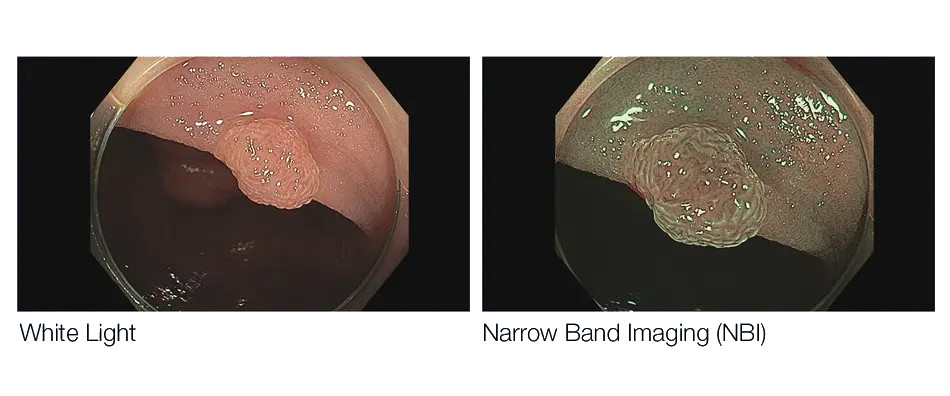
\includegraphics[width=\linewidth]{illustrations/narrow_band.jpg}
		\caption{Narrowband imaging and white-light endoscopy constitutes a distributional shift. Adapted from \cite{nbi_img}}
		\label{imaging_modalities}
	\end{figure}

	Though the features each model learns are not particularly representative of the broader context of what makes a polyp a polyp, they make sense when considered from the perspective of either of the two modalities. When considering only narrow-band imaging, it makes some sense to heavily weigh the texture of the polyps. When considering only white-light imaging, it makes some sense to heavily weight the shape and colour of the polyps. Though humans are capable of appreciating broader context and subconsciously know that certain features are ancilliary rather than causal (and perhaps more importantly: know the strengths and weaknesses of each modality), DNNs lack the inductive biases needed to take this into account. Once again, DNNs merely leverage the first and best predictive patterns found during the training process, and cannot be expected to optimize for specific invariances on their own, irrespective of how self-evident these invariances may be for humans. This predilection towards dataset-specific features is aptly referred to as dataset bias. 
	
	\subsubsection{Shortcut Learning}
	In the aforementioned example, though the features each predictor learns is not robust to dataset shift, they nevertheless have causal explanations. The causal structure that they correspond to is of course not dataset-agnostic, and as a result flawed in their own way, but the patterns the respective models leverage to interpret the data are not particularly irrational. As it turns out, however, DNNs are unlikely to learn such causally viable features in the first place. In other words, the predictors would not necessarily learn to consider texture in narrow-band images - it could learn any arbitrary pattern so long as it is predictive. Moreover, if such interpretable distributional shifts were the principal cause of generalization failure, generalizability could be practically guaranteed by explicitly modelling the effects such shifts induce and taking this into account in the pipeline. In the aforementioned example, one could for instance train some model to map from one lighting environment to the other. Though this would imbue the model with an inherent invariance to the choice of lighting, it is nonetheless not given that the resulting model will be perfectly generalizable.

	Consequently, though these detectable forms of distributional shifts also hold some importance when designing generalizable models, a more pervasive and substantially more significant issue is the fact that many of the distributional shifts encountered in clinical settings are not necessarily considered significant or for that matter at all perceptible to a human observer. A human would for instance not be significantly affected by slightly noisy, blurry, rotated, or compressed images, nor would they in all likelihood notice these perturbations. DNNs, on the other hand, have been shown to be highly sensitive to these and several other forms of minor perturbations \cite{noise_robustness, corruption_robustness,adversarial_training,benchmarking_robustness}. Moreover, a human would likely not pick up on subtle phenotypic cues that may exist in the colon during endoscopy, whereas a DNN may leverage some of these cues to inform their decisions, and hence exhibit varying performance across different demographics. 

	It is important to note, however, that despite how these two forms of distributional shift may at surface level appear as completely separate classes of problems, they can both be traced to the same phenomena - namely that DNNs do not leverage any form of causal logic to inform their decisions and, as mentioned previously, simply exploit any sufficiently predictive pattern they may observe in the data. This phenomenon has been shown to be pervasive across all manner of domains, from natural language processing and computer vision to reinforcement learning and algorithmic decision-making. This is referred to as shortcut learning \cite{shortcut_learning} or the Clever Hans effect \cite{cleverhans}. 

	Shortcut learning and the brittle features it corresponds to have also been identified as one of the key properties that explains the effectiveness and pervasiveness of adversarial attacks \cite{adversarial_bugs_features}. Naturally, a generalizable predictor should be robust to such minor perturbations, as the model should not in the first place be learning features that get perturbed to any significant degree by adding such high-frequency, low-amplitude noise. Adversarial attacks simply leverage the high degrees of sensitivity inherent to shortcut features, and construct perturbations according the direction in the search space that corresponds to the principal component of this sensitivity \cite{sensitivity}. 

	\begin{figure}[h]
		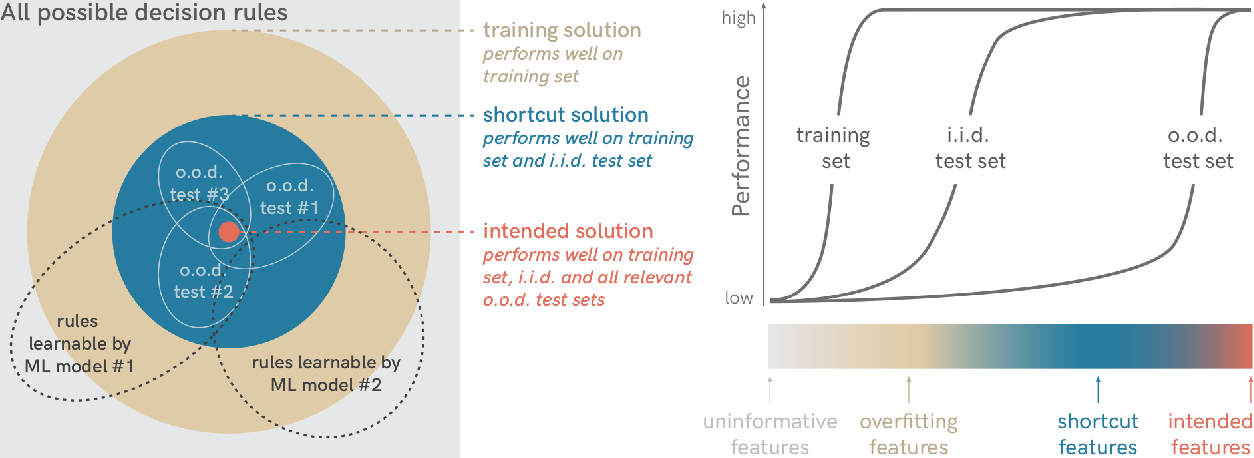
\includegraphics[width=\linewidth]{illustrations/features.png}
		\caption{Taxonomy of feature types. Adapted from \cite{shortcut_learning}}
		\label{feature_types}
	\end{figure}


	\subsection{Underspecification}
	Closely related to shortcut learning is underspecification \cite{damour2020underspecification}. A machine learning pipeline can be considered underspecified when it can return any number of risk-equivalent predictors when evaluated on an iid holdout set, dependent only on the random variables used within the training procedure - i.e dropout, seed initialization, and so on. Even with identical hyperparameters, a given training procedure can return any number of predictors each having learned different patterns. One predictor may have learned one shortcut, another may have learned a different shortcut, and one may have fully learned the actual causal relationships it is intended to. With ERM, and in particular with iid-oriented evaluation procedures, these are all erroneously considered equivalent. 

	Note that this does not however presuppose anything about the relative occurrence rates of generalizable and non-generalizable predictors. It may not necessarily even be the case that the pipeline can return a generalizable predictor at all. Only that there exists a multitude of risk-equivalent predictors in the search space the optimizer typically explores. Nor does it presuppose anything about the distribution of predictors, only that there is indeed a distribution. 

	This is evidenced by the fact that generalizability can vary greatly depending on the choice of random seed used during training. In the foundational paper on underspecification in deep learning, for instance, it was highlighted that certain classification pipelines can produce predictors that vary in ood accuracy by up to 10\% \cite{damour2020underspecification}. This is a function of the robustness of the learned features and how likely the pipeline is to return the corresponding predictors. 
	\subsection{A probabilisitic perspective of generalization}
	As established, modern deep learning pipelines are not capable of reliably returning generalizable predictors. However, they are not necessarily precluded from it. One can to some extent model this probabilistically by considering the distribution of parameters given the training data, \(p(w | \mathcal{D})\). Though it is impossible to know which part of this distribution corresponds to generalizable predictors, it has been shown that marginalizing over this distribution - in other words, bayesian learning - increases generalizability \cite{bayesian_generalization,endoensemble,divergentnets,ensemble_machinereading}. 

	\cite{bayesian_generalization} provides a probabilistic perspective of this phenomenon. They consider generalizability as a two-dimensional quantity, consisting of the support and inductive biases of a model. The inductive biases are as mentioned the constraints by which the model learns, ranging from model-construction - e.g positional invariance in CNNs - to regularization - e.g dropout, data augmentation, etc - and specific training routines - i.e multitask learning, contrastive representation learning, etc. The support, on the other hand, describes the ability of the model to encode certain decision rules. Ideally, and as is the case in deep learning, support should be maximized, as the model should be able to learn as complicated decision rules as may be required by a given problem. Similarly, and perhaps intuitively, the amount of inductive biases imposed on the model a-priori should also be maximized, as it reduces the probability of learning spurious correlations. 

\section{Related work on generalizable deep learning}
To summarize, generalization failure occurs due to the weaknesses inherent to ERM. The features that ERM learn to incorporate are often spurious, and the predictors that leverage them are often returned practically arbitrarily from the pipeline. The approaches that have exhibited the highest degrees of success towards increasing generalization as a consequence tend to address these issues in some way or another. 

One of the most well-studied approaches to increasing generalizability is the use of data augmentation. Data augmentation is typically implemented in deep learning pipelines in order to prevent overfitting, often in conjunction with other regularization methods. Naturally, overfitting also constitutes generalizability failure in its own right, but augmentation has also been shown to have positive effects for out-of-distribution generalization. It has for instance been shown that carefully designing augmentation procedures increases the generalizability of polyp segmentation models \cite{polyp_augmentation} and prostate segmentation \cite{augmentation_prostate}. There has also been a large body of work dedicated to leveraging recent advances in generative models such as generative adversarial networks (GANs) and variational autoencoders (VaEs) to serve as synthetic data augmentation. These types of approaches have also been shown to increase generalizability in CT segmentation \cite{cyclegan} and x-ray based covid detection \cite{covid}. Data augmentation facilitates generalization by implicitly biasing the pipeline towards credible inductive biases, as the empirical risk will be best minimized by leveraging features that are conducive to minimizing risk across both synthetic or otherwise augmented data and unaugmented data. Naturally, the choice of augmentations that are used is an inductive bias in and of itself; by employing random rotations, rotational invariance is presupposed. By employing random cropping, image-space object size invariance is presupposed. By employing additive noise, invariance to additive noise is presupposed, and so on. From an ERM perspective, this corresponds to improving the empirical risk estimate; given enough data, all of these invariances may be learned automatically. With a finite and often fairly limited dataset, this may not necessarily be the case simply due to the large number of confounding variables involved. 

Another type of approach involves biasing the pipeline towards learning more structured and causally viable latent representations. This is also somewhat well understood when considered through the lens of regularization: drop-out and weight-decay are often employed in order to reduce overfitting under the assumption that a generalizable predictor should not base its decisions on only a few of the available neurons and that separate neurons should instead encode independent representations of the input. Though there is limited research on the effects of dropout on ood generalization, constraining the latent representations in DNNs has been shown to be effective method to increase generalizability. For polyp-segmentation it has for instance been shown that adding context-based attention layers to multiple blocks in a given network results in state-of-the-art IoU scores for out-of-distribution evaluation on certain datasets \cite{uacanet}. Other attention-based approaches have also shown promise in this regard \cite{attention_generalizability, reverse_attention}. This permits the model to learn and generate attention maps for its latent representations, thus in theory biasing the model towards learning more a more structured interpretation of the data. 

Multi-task and/or multistage learning has also been leveraged to this end. By jointly optimizing for multiple tasks/subtasks, the model can be biased towards learning features that describe the input data well independent of their performance on any one of the relevant tasks. For polyp-segmentation, for instance, it has been shown that adding image reconstruction as an auxiliary task \cite{ddanet} or decoupling the segmentation task into a coarse segmentation and refinement stage \cite{doubleencdec} increases generalizability. 

More closely supervised methods, wherein certain inductive biases have been explicitly introduced to the pipeline, have also been shown to have some promise. One paper for instance reported an increased robustness to image perturbations after adding a custom filter bank designed to emulate the primary visual cortex of primates to the front of the CNN \cite{visual_cortex}. Another reported that models trained on imagenet exhibited significantly higher robustness when explicitly biased towards shape-based features \cite{texturebias}. 

	
These approaches all provide workarounds to flaws with ERM, typically to limited practical effect. Consequently, a growing body of work has instead been investigating the idea of foregoing ERM altogether in favour of developing alternative training paradigms. In so-called Invariant Risk Minimization\cite{IRM}, for instance, the model trains to ignore spurious correlations by optimizing for predictors that exhibit stable performance across multiple training environments. A similar approach, namely model-based robust deep learning \cite{modelbased}, employs a similar idea in conjunction with distributional modelling. The model is trained such that it is robust to perturbations as generated by a so-called model of natural variation. If this model for instance describes the function mapping one training environment to another, this will then optimize for predictors that are invariant to the distributional shift this function corresponds to. 

Finally, Bayesian learning has also been shown to improve generalization. In particular, ensemble-based networks - which mathematically can be considered an approximation of Bayesian marginalization \cite{bayesian_case,bayesian_generalization} - have demonstrated high degrees of generalizability for polyp-segmentation \cite{divergentnets,endoensemble}. Since deep learning pipelines are typically underspecified, one can consider an ensemble of predictors to be a sampling of the distribution over parameters given training data. These predictors are of course unlikely to have learned identical representations, and consequently whatever spurious correlations inferred by one predictor may be countered by the features employed in another. Consequently, features that are stable across predictors and consequently more likely to generalize are weighed to a greater extent, in turn mitigating the effects of underspecification. Structural misalignment may nevertheless impact ensembles, and as such the effective returns are limited. 

